% Options for packages loaded elsewhere
\PassOptionsToPackage{unicode}{hyperref}
\PassOptionsToPackage{hyphens}{url}
\PassOptionsToPackage{dvipsnames,svgnames,x11names}{xcolor}
%
\documentclass[
sn-nature
]{sn-jnl}

\usepackage{amsmath,amssymb}
\usepackage{iftex}
\ifPDFTeX
  \usepackage[T1]{fontenc}
  \usepackage[utf8]{inputenc}
  \usepackage{textcomp} % provide euro and other symbols
\else % if luatex or xetex
  \usepackage{unicode-math}
  \defaultfontfeatures{Scale=MatchLowercase}
  \defaultfontfeatures[\rmfamily]{Ligatures=TeX,Scale=1}
\fi
\usepackage{lmodern}
\ifPDFTeX\else  
    % xetex/luatex font selection
\fi
% Use upquote if available, for straight quotes in verbatim environments
\IfFileExists{upquote.sty}{\usepackage{upquote}}{}
\IfFileExists{microtype.sty}{% use microtype if available
  \usepackage[]{microtype}
  \UseMicrotypeSet[protrusion]{basicmath} % disable protrusion for tt fonts
}{}
\makeatletter
\@ifundefined{KOMAClassName}{% if non-KOMA class
  \IfFileExists{parskip.sty}{%
    \usepackage{parskip}
  }{% else
    \setlength{\parindent}{0pt}
    \setlength{\parskip}{6pt plus 2pt minus 1pt}}
}{% if KOMA class
  \KOMAoptions{parskip=half}}
\makeatother
\usepackage{xcolor}
\setlength{\emergencystretch}{3em} % prevent overfull lines
\setcounter{secnumdepth}{-\maxdimen} % remove section numbering
% Make \paragraph and \subparagraph free-standing
\makeatletter
\ifx\paragraph\undefined\else
  \let\oldparagraph\paragraph
  \renewcommand{\paragraph}{
    \@ifstar
      \xxxParagraphStar
      \xxxParagraphNoStar
  }
  \newcommand{\xxxParagraphStar}[1]{\oldparagraph*{#1}\mbox{}}
  \newcommand{\xxxParagraphNoStar}[1]{\oldparagraph{#1}\mbox{}}
\fi
\ifx\subparagraph\undefined\else
  \let\oldsubparagraph\subparagraph
  \renewcommand{\subparagraph}{
    \@ifstar
      \xxxSubParagraphStar
      \xxxSubParagraphNoStar
  }
  \newcommand{\xxxSubParagraphStar}[1]{\oldsubparagraph*{#1}\mbox{}}
  \newcommand{\xxxSubParagraphNoStar}[1]{\oldsubparagraph{#1}\mbox{}}
\fi
\makeatother


\providecommand{\tightlist}{%
  \setlength{\itemsep}{0pt}\setlength{\parskip}{0pt}}\usepackage{longtable,booktabs,array}
\usepackage{calc} % for calculating minipage widths
% Correct order of tables after \paragraph or \subparagraph
\usepackage{etoolbox}
\makeatletter
\patchcmd\longtable{\par}{\if@noskipsec\mbox{}\fi\par}{}{}
\makeatother
% Allow footnotes in longtable head/foot
\IfFileExists{footnotehyper.sty}{\usepackage{footnotehyper}}{\usepackage{footnote}}
\makesavenoteenv{longtable}
\usepackage{graphicx}
\makeatletter
\def\maxwidth{\ifdim\Gin@nat@width>\linewidth\linewidth\else\Gin@nat@width\fi}
\def\maxheight{\ifdim\Gin@nat@height>\textheight\textheight\else\Gin@nat@height\fi}
\makeatother
% Scale images if necessary, so that they will not overflow the page
% margins by default, and it is still possible to overwrite the defaults
% using explicit options in \includegraphics[width, height, ...]{}
\setkeys{Gin}{width=\maxwidth,height=\maxheight,keepaspectratio}
% Set default figure placement to htbp
\makeatletter
\def\fps@figure{htbp}
\makeatother
% definitions for citeproc citations
\NewDocumentCommand\citeproctext{}{}
\NewDocumentCommand\citeproc{mm}{%
  \begingroup\def\citeproctext{#2}\cite{#1}\endgroup}
\makeatletter
 % allow citations to break across lines
 \let\@cite@ofmt\@firstofone
 % avoid brackets around text for \cite:
 \def\@biblabel#1{}
 \def\@cite#1#2{{#1\if@tempswa , #2\fi}}
\makeatother
\newlength{\cslhangindent}
\setlength{\cslhangindent}{1.5em}
\newlength{\csllabelwidth}
\setlength{\csllabelwidth}{3em}
\newenvironment{CSLReferences}[2] % #1 hanging-indent, #2 entry-spacing
 {\begin{list}{}{%
  \setlength{\itemindent}{0pt}
  \setlength{\leftmargin}{0pt}
  \setlength{\parsep}{0pt}
  % turn on hanging indent if param 1 is 1
  \ifodd #1
   \setlength{\leftmargin}{\cslhangindent}
   \setlength{\itemindent}{-1\cslhangindent}
  \fi
  % set entry spacing
  \setlength{\itemsep}{#2\baselineskip}}}
 {\end{list}}
\usepackage{calc}
\newcommand{\CSLBlock}[1]{\hfill\break\parbox[t]{\linewidth}{\strut\ignorespaces#1\strut}}
\newcommand{\CSLLeftMargin}[1]{\parbox[t]{\csllabelwidth}{\strut#1\strut}}
\newcommand{\CSLRightInline}[1]{\parbox[t]{\linewidth - \csllabelwidth}{\strut#1\strut}}
\newcommand{\CSLIndent}[1]{\hspace{\cslhangindent}#1}

%%%% Standard Packages

\usepackage{graphicx}%
\usepackage{multirow}%
\usepackage{amsmath,amssymb,amsfonts}%
\usepackage{amsthm}%
\usepackage{mathrsfs}%
\usepackage[title]{appendix}%
\usepackage{xcolor}%
\usepackage{textcomp}%
\usepackage{manyfoot}%
\usepackage{booktabs}%
\usepackage{algorithm}%
\usepackage{algorithmicx}%
\usepackage{algpseudocode}%
\usepackage{listings}%

%%%%

\raggedbottom
\usepackage{booktabs}
\usepackage{longtable}
\usepackage{array}
\usepackage{multirow}
\usepackage{wrapfig}
\usepackage{float}
\usepackage{colortbl}
\usepackage{pdflscape}
\usepackage{tabu}
\usepackage{threeparttable}
\usepackage{threeparttablex}
\usepackage[normalem]{ulem}
\usepackage{makecell}
\usepackage{xcolor}
\makeatletter
\@ifpackageloaded{caption}{}{\usepackage{caption}}
\AtBeginDocument{%
\ifdefined\contentsname
  \renewcommand*\contentsname{Table of contents}
\else
  \newcommand\contentsname{Table of contents}
\fi
\ifdefined\listfigurename
  \renewcommand*\listfigurename{List of Figures}
\else
  \newcommand\listfigurename{List of Figures}
\fi
\ifdefined\listtablename
  \renewcommand*\listtablename{List of Tables}
\else
  \newcommand\listtablename{List of Tables}
\fi
\ifdefined\figurename
  \renewcommand*\figurename{Figure}
\else
  \newcommand\figurename{Figure}
\fi
\ifdefined\tablename
  \renewcommand*\tablename{Table}
\else
  \newcommand\tablename{Table}
\fi
}
\@ifpackageloaded{float}{}{\usepackage{float}}
\floatstyle{ruled}
\@ifundefined{c@chapter}{\newfloat{codelisting}{h}{lop}}{\newfloat{codelisting}{h}{lop}[chapter]}
\floatname{codelisting}{Listing}
\newcommand*\listoflistings{\listof{codelisting}{List of Listings}}
\makeatother
\makeatletter
\makeatother
\makeatletter
\@ifpackageloaded{caption}{}{\usepackage{caption}}
\@ifpackageloaded{subcaption}{}{\usepackage{subcaption}}
\makeatother
\ifLuaTeX
  \usepackage{selnolig}  % disable illegal ligatures
\fi
\usepackage{bookmark}

\IfFileExists{xurl.sty}{\usepackage{xurl}}{} % add URL line breaks if available
\urlstyle{same} % disable monospaced font for URLs
\hypersetup{
  pdftitle={The Application of Magnetic Susceptibility Separation for Measuring Cerebral Oxygenation in Preterm Neonates},
  pdfauthor={Thomas Gavin Carmichael; Alexander Rauscher; Ruth E Grunau; Alexander Mark Weber},
  pdfkeywords={Quantitative Susceptbility
Mapping, Preterm, Newborn, Cerebral Venous Oxygen Saturation},
  colorlinks=true,
  linkcolor={blue},
  filecolor={Maroon},
  citecolor={Blue},
  urlcolor={Blue},
  pdfcreator={LaTeX via pandoc}}

\title[The Application of Magnetic Susceptibility Separation for
Measuring Cerebral Oxygenation in Preterm Neonates]{The Application of
Magnetic Susceptibility Separation for Measuring Cerebral Oxygenation in
Preterm Neonates}

% author setup
\author[1,2]{\fnm{Thomas Gavin} \sur{Carmichael}}\email{tgcarmichael@outlook.com}\author[3]{\fnm{Alexander} \sur{Rauscher}}\email{rauscher@physics.ubc.ca}\author[2,3]{\fnm{Ruth E} \sur{Grunau}}\email{rgrunau@mail.ubc.ca}\author*[2,3]{\fnm{Alexander Mark} \sur{Weber}}\email{aweber@bcchr.ca}
% affil setup
\affil[1]{\orgdiv{Integrated Sciences}, \orgname{The University of
British Columbia}, \orgaddress{\street{2329 West
Mall}, \city{Vancouver}, \postcode{V6T 1Z4}, \country{Canada}}}
\affil[3]{\orgdiv{Pediatrics}, \orgname{The University of British
Columbia}, \orgaddress{\street{2329 West
Mall}, \city{Vancouver}, \postcode{V6T 1Z4}, \country{Canada}}}
\affil[2]{\orgdiv{BC Children's Hospital Research
Institute}, \orgname{The University of British
Columbia}, \orgaddress{\street{938 West 28th
Avenue}, \city{Vancouver}, \postcode{V5Z 4H4}, \country{Canada}}}

% abstract 

\abstract{\textbf{Background}: Quantitative susceptibility mapping (QSM)
is a magnetic resonance imaging (MRI) modality proposed to be a viable
method of measuring cerebral oxygenation in neonates given its
sensitivity to deoxyhemoglobin, a paramagnetic molecule. During QSM,
however, paramagnetic sources can be obscured by opposing diamagnetic
sources such as water and myelin. We sought to evaluate whether QSM
images alone, or an algorithm that attempts to isolate their
paramagnetic components, are more accurate in measuring oxygenation of
the major cerebral veins in a cohort of neonates born preterm.
Additionally, we aimed to determine whether a difference in oxygenation
existed between the major cerebral veins.

\textbf{Methods}: 19 neonates born preterm were scanned on a 3T research
MRI at term equivalent age. The protocol included a multi-echo
susceptibility-weighted imaging sequence. The acquired imaging data were
processed as QSM images to obtain the susceptibility values of the
superior sagittal sinus (SSS) and central cerebral veins (CCV). These
values were used to calculate the oxygen saturation
(SvO\textsubscript{2}) of the SSS and CCV. QSM images were subsequently
processed to isolate their paramagnetic components. SvO\textsubscript{2}
values of the SSS and CCV were calculated again from the paramagnetic
components.

\textbf{Results}: The mean SvO\textsubscript{2} values of the SSS and
CCV calculated from QSM images were found to be 72.4\% (SD, 3.4\%) and
68.7\% (SD, 3.5\%), respectively. The mean SvO\textsubscript{2} values
calculated from paramagnetic components were found to be 58.1\% (SD,
7.3\%) for the SSS and 57.7\% (SD, 7.0\%) for the CCV.

\textbf{Conclusion}: SSS SvO\textsubscript{2} values derived from
paramagnetic components agreed well with the existing literature and
were closer than the values derived from QSM, however, they displayed
greater variability. Although the CCV SvO\textsubscript{2} data from QSM
aligns more closely with existing literature, it is important to note
that the current literature on this topic remains relatively limited in
the CCV. Thus, decomposing QSM images into paramagnetic components shows
great promise as a method for more accurately measuring cerebral
oxygenation in neonates but may require more research to improve
precision. Notably, no significant difference in oxygenation was
observed between the CCV and the SSS, contrasting with previous
studies.}

% keywords
\keywords{Quantitative Susceptbility
Mapping,  Preterm,  Newborn,  Cerebral Venous Oxygen Saturation}

\begin{document}
\maketitle

\section{Introduction}\label{sec-intro}

Preterm birth

Abnormal brain development is a significant concern for parents with
children born preterm, as 43\% of infants that survive will have
neurodevelopmental delays later in life (Dix, van Bel, and Lemmers
2017). Irregularities in early cerebral oxygen levels have been
identified as a potential source of such delays, where too little oxygen
provided during NICU care can result in white matter injury, while too
much oxygen can result in reduced cortical connectivity (Rantakari et
al. 2021). As such, being able to precisely, accurately, and
non-invasively measure cerebral oxygenation is necessary for
understanding and improving neurodevelopmental outcomes in preterm
neonates.

In the present study, we set out to determine whether a QSM image alone,
or the paramagnetic component of the QSM image, is more accurate in
measuring the oxygen present in the major cerebral veins of a cohort of
preterm neonates. As previous QSM studies have not included the SSS, we
also had a secondary aim of preserving this vessel in our QSM images and
using this data to determine whether a difference in oxygenation existed
between the SSS and the central cerebral veins (CCV).

\section{Methods}\label{sec-data-methods}

The study was approved by the Clinical Research Ethics Board at the
University of British Columbia and Children's \& Women's Hospital
(H21-00655) and written informed consent was obtained from the
parent/guardian for each infant.

\subsection{Study population}\label{study-population}

Participant data comes from a previous study (Zhu et al. 2024).
Participants consisted of preterm neonates born between 25- and 31-weeks
gestational age (GA) who were admitted to the level III NICU at BC
Women's Hospital. Recruitment took place over a span of one year, from
February 2021 to January 2022, facilitated by a dedicated research
nurse. Parents of eligible infants were approached by the research nurse
prior to discharge from the NICU to explain the study objectives and
seek their consent for participation. Infants meeting the criteria for
inclusion were scanned for the study if they had already been discharged
from the NICU, were in stable condition, and had reached a term
equivalent age of 37 to 44 weeks GA. However, certain exclusion criteria
were applied to ensure the homogeneity and integrity of the study
sample. Infants were excluded if there was clinical evidence of a
congenital malformation or syndrome, a TORCH infection, or ultrasound
evidence of large parenchymal hemorrhagic infarction (\textgreater2 cm,
Grade 4 intraventricular hemorrhage).

\subsection{Image acquisition}\label{image-acquisition}

MR imaging was performed on a 3.0 Tesla General Electric Discovery MR750
scanner (scanner software version DV26.0\_R03) equipped with a SREE
Medical Systems single-channel neonatal head coil (Table~\ref{tbl-mri}).
The scans were conducted at the BC Children's MRI Research Facility.
Prior to the scanning procedure, subjects were carefully prepared by a
research nurse. Swaddling and feeding were used to ensure the comfort
and cooperation of the subjects during the scan. Importantly, no
sedatives or invasive markers were utilized throughout the procedure.
Subjects were placed within a specially designed SREE Medical Systems
MRI compatible incubator, which facilitated both safety and motion
minimization. Molded foam was strategically positioned around the head
and body within the incubator to further restrict subject movement. To
protect against potential hearing damage, ear plugs were employed during
the scanning process. Additionally, a pulse oximeter was affixed to the
subject's foot to monitor arterial oxygen saturation and heart rate
throughout the scan.

\begin{table}

\caption{\label{tbl-mri}Technical parameters for MR imaging pulse
sequences}

\centering{

    \begin{tabular*}{\textwidth}{@{}p{2.5cm}llp{2.5cm}p{2.5cm}@{}}
    \toprule
        ~ & T1w & T2w & pcASL & SWI \\ \midrule
        Sequence & 3D FSPGR & 3D CUBE & Multi-shot 3D fast spin-echo & 3D spoiled GRE flow-compensated \\
        Phase-encoding direction & Coronal & Sagittal & Axial & Axial \\
        TR (ms) & 7.74 & 2,300 & 4,680 & 30.9 \\
        TE (ms) & 2.97 & 66.29 & 10.55 & 5.24 \\
        Flip angle & 12$^{\circ}$ & 90$^{\circ}$ & 111$^{\circ}$ & 20$^{\circ}$ \\
        FOV (cm) & 20 & 20 & 24 & 25 \\
        Acquisition matrix & 512 x 512 & 256 x 256 & 128 x 128 & 256 x 256 \\
        In-plane resolution (mm) & 0.39 x 0.39 & 0.78 x 0.78 & 1.875 x 1.875 & 0.977 x 0.977 \\
        Slice thickness (mm) & 1 & 1 & 4 & 2, reconstructed to 1 with zero filling (ZIP2) \\
        Number of slices & 126 & 106 & 50 & 92 \\
        Additional parameters & n/a & n/a & 1,450 ms label period; 2,025 ms pulse label; 24 control-label pairs & n/a \\
        Scan duration & 4 min 39 s & 5 min 1 s & 5 min 26 s & 5 min 29 s \\ \botrule
    \end{tabular*}
    \footnotetext{T1w = T1-weighted; T2w = T2-weighted; pcASL = pseudo-continuous arterial spin labelling; SWI = susceptibility weighted imaging; FSPG = fast spoiled gradient echo; CUBE = General Electric name of sequence, not an acronym; GRE = gradient echo; ZIP2 = through-plane zero filling interpolation}

}

\end{table}%

The MRI scan protocol comprised of the following sequences: a
T1-weighted scan, a T2-weighted scan, a pseudo-continuous arterial spin
labeling (ASL) scan, a multi-echo susceptibility-weighted imaging scan,
and a diffusion-weighted imaging (DWI) spin-echo echo planar imaging
(EPI) sequence. The DWI sequence was not used for the present study.

\subsection{Image analysis}\label{image-analysis}

The raw DICOM files acquired from the scanning procedure were converted
to NIfTI (Neuroimaging Informatics Technology Initiative) format using
Chris Rorden's \texttt{dcmniix} tool. SWI magnitude data files were then
used to create subject-specific brain masks that would not erode the SSS
during QSM processing, an issue faced by our group in the past (X. Li et
al. 2016). A step-by-step summary of the pipeline used is shown in
Figure~\ref{fig-sample}.

\begin{figure}[H]

\centering{

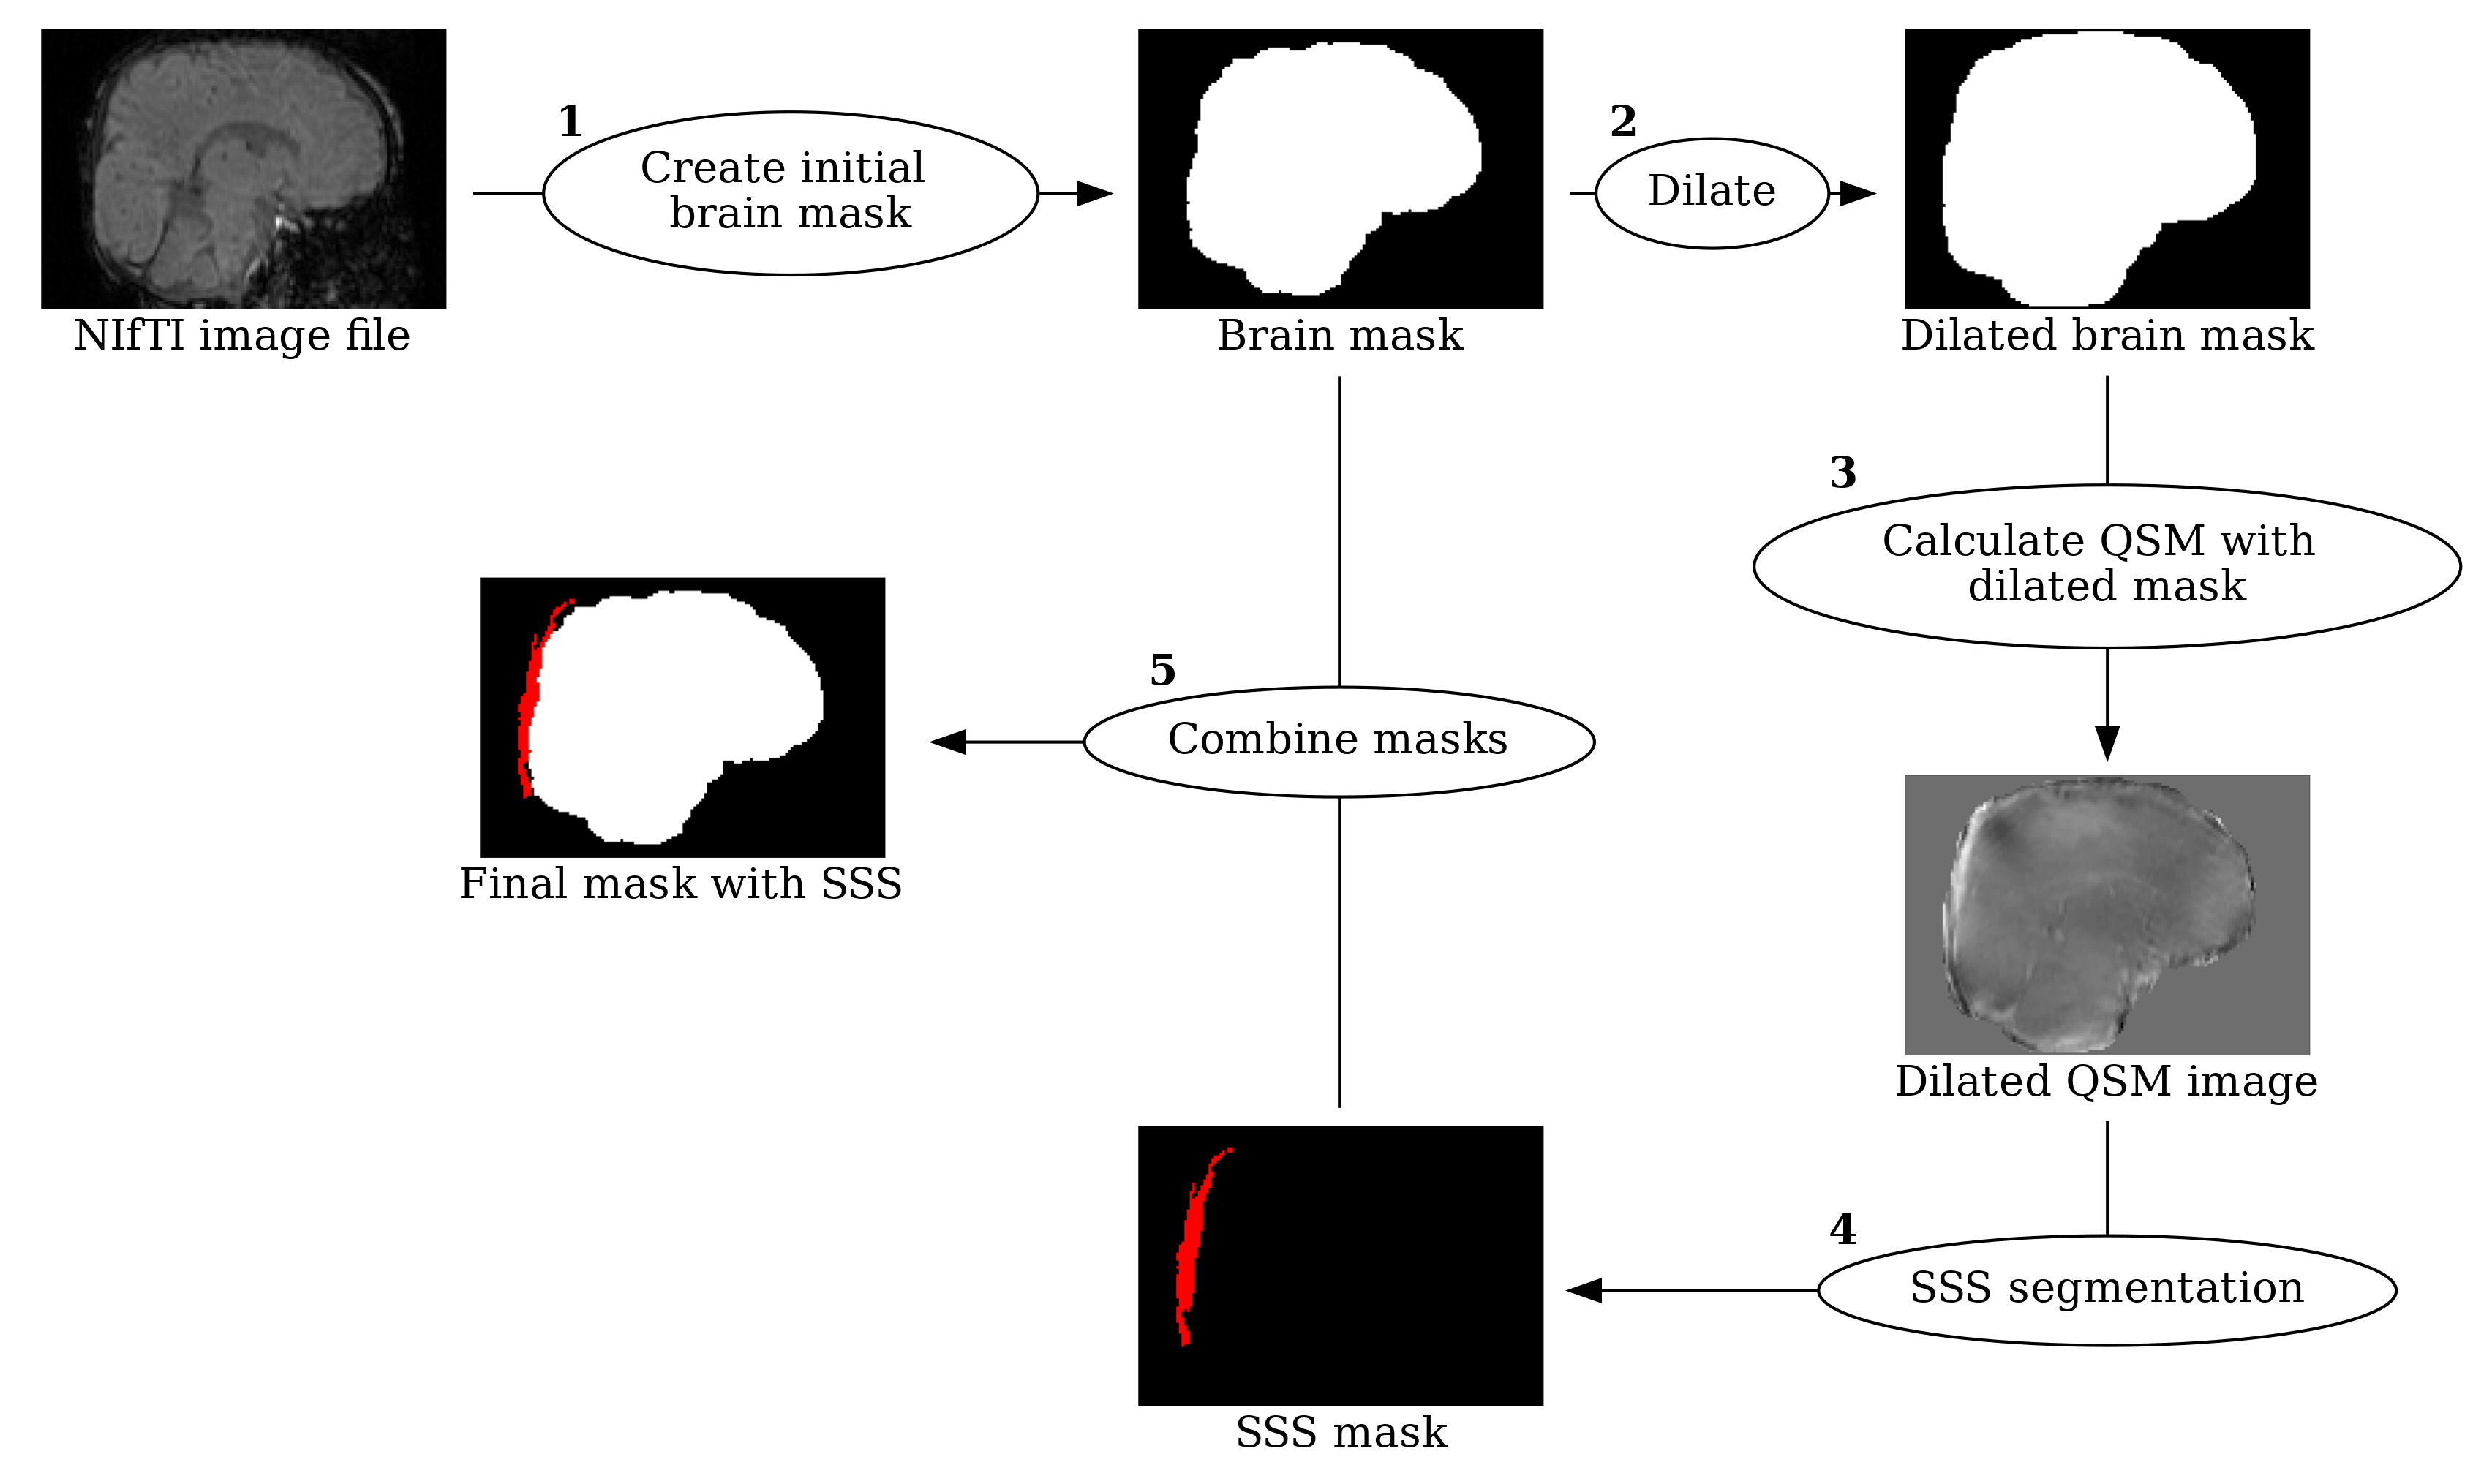
\includegraphics{index_files/figure-latex/notebooks-Figures-fig-graph-output-1.png}

}

\caption{\label{fig-graph}Pipeline for generating subject-specific brain
masks that include the superior sagittal sinus (SSS). Initial steps
involved (1) creating brain a mask from the magnitude of the fifth echo
of the susceptibility weighted scan. Subsequently, the brain mask is
dilated and then (2) utilized in conjunction with a quantitative
susceptibility mapping (QSM) script to generate a preliminary QSM image.
Further refinement involved (3) segmenting the SSS from the QSM image
manually to create a tissue mask of the SSS region. Finally, (4) the
vascular mask of the SSS is integrated with the initial brain mask,
forming the comprehensive brain mask essential for obtaining
susceptibility data that includes the SSS.}

\end{figure}%

First, the fifth echo SWI magnitude file was processed using FSL's (v.
6.0.7.3) (Woolrich et al. 2009) \texttt{fslroi}, \texttt{fslmaths}, and
\texttt{bet} (Smith 2002) to create a preliminary brain mask, similar to
our previous efforts, which does not contain the SSS. \texttt{Fslroi}
was used to isolate the fifth echo of the magnitude data, which was then
squared using Fslmaths and the option \texttt{-sqr}. Squaring the
magnitude image was found to dramatically improve subsequent brain
extraction. The resulting image was then used to create the preliminary
brain mask using bet with the options \texttt{-m} and \texttt{-R}. The
former flag generated a binary brain mask, while the latter performed a
more robust brain centre estimation. The brain mask was then dilated by
7 voxels using \texttt{Fslmaths} and the options \texttt{-kernel\ boxv}
and \texttt{-dilM} in order for the dilated mask to contain the SSS
(along with unwanted tissue as well). This mask was then used, along
with the phase images, in a MATLAB script for QSM calculation from
Christian Kames (Kames, Wiggermann, and Rauscher 2018) to produce a
preliminary QSM image that contained the SSS, albeit with fairly low
signal-to-noise ratio and other unwanted tissue. Given the high contrast
in voxel intensity between the SSS and surrounding tissue, the select by
intensity tool in \texttt{FSLeyes} (McCarthy 2023) was then used to
segment the SSS from the QSM image and create a 3D mask of the selected
region. Using \texttt{fslmaths} and the options \texttt{-add} and
\texttt{-bin}, the SSS mask was then combined with the original brain
mask of the fifth echo. This resulted in a brain mask that contained
only brain and SSS signal. Finally, this mask was used in a final QSM
post-processing step to create a QSM image that includes the SSS while
maintaining a high signal-to-noise ratio, making it suitable to obtain
accurate susceptibility values.

STI Suite (v. 3.0) (W. Li et al. 2014), was used to process the final
QSM images as it produced the cleanest images without eroding the SSS.
The finalized brain mask and the last three echoes of the magnitude and
phase images were used in STI Suite along with the following parameters:
0.9766 x 0.9766 x 1 mm\textsuperscript{3} voxel size, 5 ms TE1, 5.3 ms
\(\Delta\)TE, and 77.4 ms sum TE, B0 strength = 3, and B0 direction =
{[}0, 0, 1{]}. The 3D GRE data option was selected for the phase
processing stage, and STAR-QSM was selected for the QSM stage. Finally,
the `select by intensity' tool in \texttt{FSLeyes} was then used to
semi-automatically make vascular masks of the SSS and CCV from each
subject's QSM image. The vascular masks were used to calculate the mean
susceptibility of each subject's SSS and CCV from their QSM image with
\texttt{fslstats}.

To isolate the paramagnetic component of subjects' QSM data, the
\(\chi\)-separation toolbox (Shin et al. 2021) from the Laboratory for
Imaging Science and Technology was used. Each subject's magnitude and
phase SWI data were used along with the following parameters: 0.9766 x
0.9766 x 1 mm\textsuperscript{3} voxel size; TE (s) = {[}0.005, 0.0102,
0.0155, 0.0207, 0.026{]}; delta TE (s) = 0.0052; B0 strength = 3; B0
direction = {[}0, 0, 1{]}. The mean susceptibility of each subject's SSS
and CCV in their paramagnetic maps was calculated with the same vascular
masks used for the QSM images. Sample images showing the magnitude,
final QSM, and final paramagnetic component images are shown in
Figure~\ref{fig-sample}.

\begin{figure}[H]

\centering{

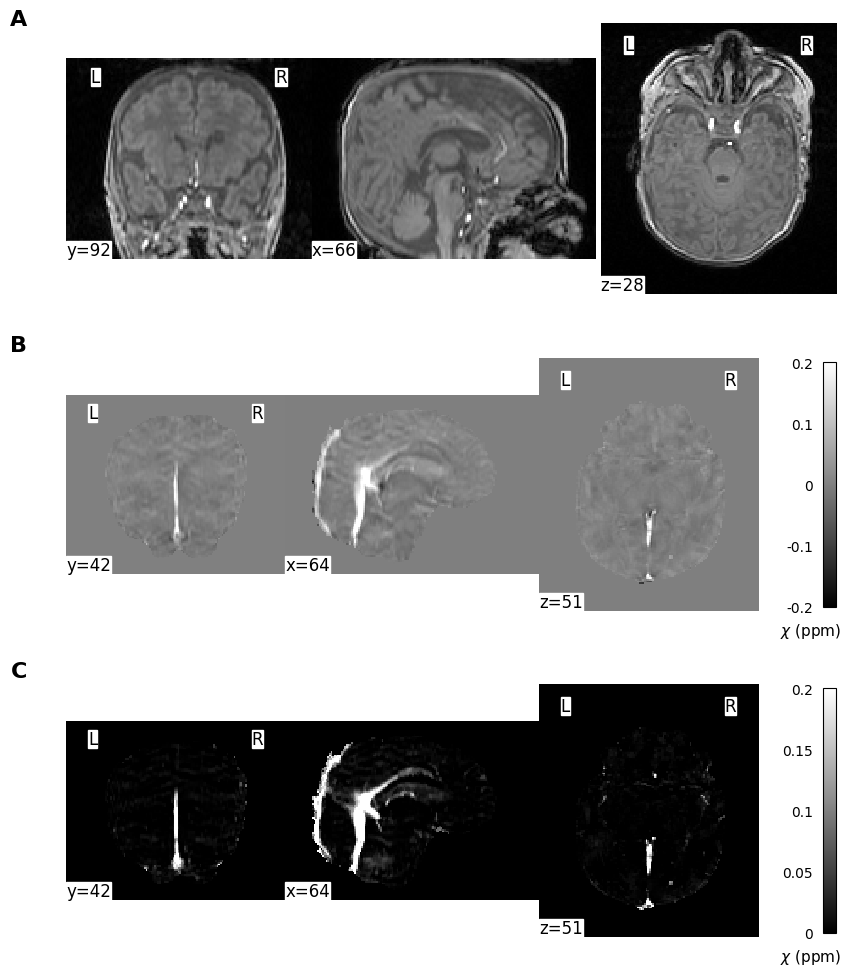
\includegraphics{index_files/figure-latex/notebooks-Figures-fig-sample-output-1.png}

}

\caption{\label{fig-sample}An example of subject imaging data. A sample
sagittal, coronal, and axial slice is displayed for each image. (a) The
1st echo of the magnitude susceptibility weighted imaging sequence; (b)
the final quantitative susceptibility mapping image; and (c) the
paramagnetic component isolated from the quantitative susceptibility
map. The bars in (b) and (c) indicates the range of susceptibility
\(\chi\) values.}

\end{figure}%

Once the mean susceptibility values of the SSS and CCV were obtained
from the subjects' QSM images and paramagnetic maps, venous oxygen
saturation (SvO\textsubscript{2}) was calculated with the following
equation (Berg et al. 2021):

\begin{equation}\phantomsection\label{eq-svo}{
SvO_{2} = 1 - \frac{\Delta \chi _{blood} - (\Delta \chi _{oxy} * Hct)}{\Delta \chi _{do} * Hct}
}\end{equation}

where \(\Delta \chi _{blood}\) is the vessel's measured susceptibility,
\(\Delta \chi _{oxy}\) is the constant representing the susceptibility
changes of oxygenated blood relation to water, \(\Delta \chi _{do}\) is
the difference in susceptibility between oxygenated and deoxygenated
blood, and Hct is the subject's hematocrit. \(\Delta \chi _{oxy}\) was
-0.21 * 4\(\pi\) ppm as per Portnoy et al. (2018) and (Sedlacik,
Rauscher, and Reichenbach 2007), while \(\Delta \chi _{do}\) was -0.03 *
4\(\pi\) ppm as per (Weisskoff and Kiihne 1992). Subjects' Hct for the
day of the scan was calculated using a four-parameter Weibull function
with previously measured values while still in the NICU.

\subsection{Statistical analysis}\label{statistical-analysis}

Statistical analysis of the acquired data was performed using R and
RStudio (v. 2023.09.1 Build 494) (R Core Team 2022; RStudio Team, n.d.).
Mean and standard deviation values are reported for most statistics,
unless specified otherwise. A paired Student's t-test was used to
determine statistical significance (p \textless0.05) between two
parameters (e.g.~\(\chi\) values between venous structures).

\section{Results}\label{sec-results}

A total sample size of 19 infants were scanned, with a mean (\(\pm\)
standard deviation) gestational age of 28.8 \(\pm\) 1.68 weeks and a
mean birth weight of 1276.05 \(\pm\) 294.87 grams. A comprehensive
summary of neonatal characteristics, including additional demographic
and clinical data, is provided in Table~\ref{tbl-dem} for reference.

\begin{table}

\caption{\label{tbl-dem}Demographic and clinical characteristic of the
study sample.}

\centering{

\begin{tabular}{@{}ll@{}}
    \toprule
Variable & Subject Data (n=19) \\
  \midrule
Gestational age, weeks (mean $\pm$ SD)                       & 28.8 $\pm$ 1.68                                                     \\
Corrected gestational age on scan day, weeks (mean $\pm$ SD) & 40.36 $\pm$ 1.4                                 \\
Number of male neonates (%)                                  & 10 (52.63)                          \\
Birth weight, g (mean $\pm$ SD)                              & 1276.05 $\pm$ 294.87                                                     \\
Weight on scan day, g (mean $\pm$ SD)                        & 3396.58 $\pm$ 597.72 \\
Days spent in NICU (median, IQR)                             & 53, 23                                               \\
Days on ventilation (median, IQR)                            & 31, 28.5                                 \\
\botrule
\end{tabular}
\footnotetext{SD = standard deviation; IQR = inter quartile range}

}

\end{table}%

The mean SvO\textsubscript{2} values for the SSS and the CCV were found
to be 0.72 \(\pm\) 0.03 and 0.69 \(\pm\) 0.03 ppm, respectively, when
determined from the QSM data. When determined from the paramagnetic map,
the mean SvO\textsubscript{2} values for the SSS and the CCV were found
to be 0.58 \(\pm\) 0.07 \%, respectively. A summary of the measured
physiological parameters, including the chi values used to calculate
SvO\textsubscript{2}, can found in Table~\ref{tbl-chistats}.

\begin{table}

\caption{\label{tbl-chistats}Summary of acquired physiological
parameters. Mean ± SD is shown for chi and SvO\textsubscript{2} values.
The P-value and 95\% confidence interval (CI) were obtained through the
comparison of values between QSM and paramagnetic maps; (n=19).}

\centering{

    \begin{tabular}{@{}lllp{2cm}ll@{}}
    \toprule
        Region & Measure & QSM & Paramagnetic map & p-value & 95\% CI \\ \midrule
        \multirow{ 2}{*}{SSS} & Chi (ppm)     & 0.1 \pm 0.02                     & 0.21 \pm 0.05                     & \ensuremath{2.84\times 10^{-11}}                        & -0.13, -0.09           \\
                              & SvO$_{2}$(\%) & 72.46 \pm 3.43 & 58.14 \pm 7.3 & \ensuremath{6.12\times 10^{-10}} & 11.78, 16.85 \\
        \multirow{ 2}{*}{CCV} & Chi (ppm)     & 0.13 \pm 0.02             & 0.22 \pm 0.05             & \ensuremath{6.25\times 10^{-9}}                        & -0.1, -0.07           \\
                              & SvO$_{2}$(\%) & 68.71 \pm 3.46 & 57.69 \pm 6.97 & \ensuremath{2.16\times 10^{-9}} & 8.9, 13.13 \\
        \botrule
    \end{tabular}
    \footnotetext{QSM = quantitative susceptibility mapping; CI = confidence interval; SSS = superior sagitall sinus; CCV = central cerebral vein}

}

\end{table}%

Region-specific \(\chi\) and SvO\textsubscript{2} values acquired from
QSM were compared to values acquired from paramagnetic maps. In both the
SSS and CCV, it was found that a significant difference existed between
values acquired (\(\chi\) and SvO\textsubscript{2}) from QSM and
paramagnetic maps (p \textless{} 0.05). A boxplot showing the
comparisons made is shown in Figure~\ref{fig-methodplot}.

\begin{figure}[H]

\centering{

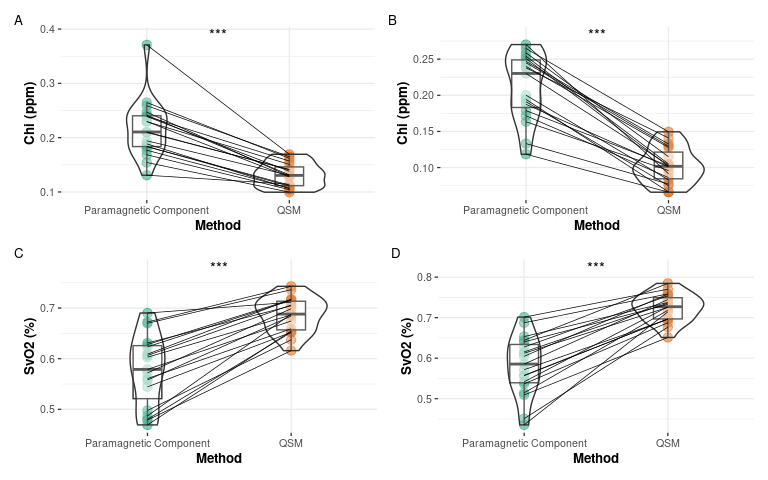
\includegraphics{index_files/figure-latex/notebooks-gavin_thesis_markdown-fig-methodplot-output-1.png}

}

\caption{\label{fig-methodplot}Vein-specific susceptibility and oxygen
saturation values by method. (A, B) contains violin plots comparing
subject χ (ppm) acquired from QSM (A) and its paramagnetic component
(B); (C, D) contains violin plots comparing subject SvO2 (\%) acquired
from QSM (C) and its paramagnetic component (D). Raw data points from
paramagnetic maps are shown as filled green circles and raw data points
from QSM are shown as filled orange circles. Each line connects the raw
data points of a single subject. (***) indicates P\textless0.05.}

\end{figure}%

The acquired \(\chi\) and SvO\textsubscript{2} values were additionally
compared between veins. In data created from QSM, a significant
difference was found between the CCV and SSS in mean \(\chi\) (p
\textless{} 0.05; 95\% CI {[}0.017, 0.04{]}) and mean
SvO\textsubscript{2} (p \textless{} 0.05; 95\% CI {[}-0.052, -0.023{]}).
In data acquired from paramagnetic maps, no significant difference was
observed between the CCV and the SSS in either mean \(\chi\) (p = 0.711;
95\% CI {[}-0.02, 0.029{]}) or mean SvO\textsubscript{2} (p = 0.752;
95\% CI {[}-0.034, 0.029{]}). A summary of these comparisons is
represented in Figure~\ref{fig-regionplot}.

\begin{figure}[H]

\centering{

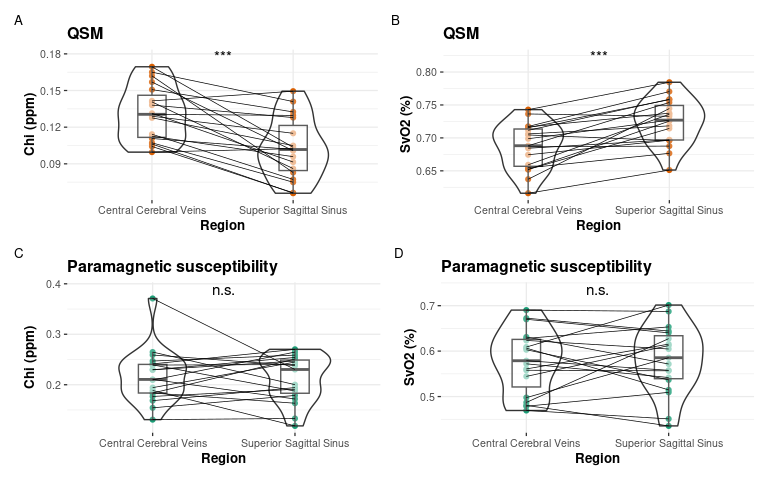
\includegraphics{index_files/figure-latex/notebooks-gavin_thesis_markdown-fig-regionplot-output-1.png}

}

\caption{\label{fig-regionplot}Inter-venous comparisons of
susceptibility and oxygen saturation. Violin plots comparing (A, C) χ
(ppm) and (B, D) SvO2 (\%) between the CCV and the SSS. Panels (A) and
(B) used data acquired from QSM, and its raw data points are shown as
filled orange circles. Panels (C) and (D) used data acquired from
paramagnetic maps, and its raw data points are shown as filled green
circles. Each line connects the raw data points of a single subject.
(***) indicates p\textless0.05; (n.s.) indicates no significant
difference.}

\end{figure}%

\section{Discussion}\label{sec-discussion}

The primary objective of the present study was to assess whether the
application of magnetic susceptibility separation to neonatal QSM data
could provide more accurate cerebral venous vessel oxygenation
measurements. To the best of our knowledge, we are the first to test
this in a neonatal cohort, as susceptibility separation has been
typically evaluated as a method of imaging myelin and brain iron in
adult subjects (Shin et al. 2021; Ahmed et al. 2023). Our results showed
that the SvO\textsubscript{2} values of the SSS and CCV obtained from
susceptibility separation are significantly lower than the respective
SvO\textsubscript{2} values obtained from QSM alone. When our results
were compared to the literature, we found that our SSS
SvO\textsubscript{2} data from susceptibility separation agreed well
with the findings of other studies measuring SvO\textsubscript{2} of the
SSS in similar subject populations. Conversely, the paramagnetic CCV
SvO\textsubscript{2} data saw less agreement with the existing
literature than the corresponding data from QSM. However, there is
reason to believe our paramagnetic CCV values may be accurate given
their similarity to the paramagnetic SSS values and the limitations of
the two studies that observed CCV SvO\textsubscript{2}. Additionally, it
is important to note that our SvO\textsubscript{2} measurements from
susceptibility separation had greater variance than our measurements
from QSM, indicating a limitation that should be addressed in future
research. Overall, the present work demonstrates the promise of
susceptibility separation as an MRI post-processing technique that can
measure the oxygenation of the cerebral veins of infant subjects, a
useful marker of regional oxygen consumption in the brain.

\section{Conclusion}\label{sec-conclusion}

\section*{References}\label{references}
\addcontentsline{toc}{section}{References}

\phantomsection\label{refs}
\begin{CSLReferences}{1}{0}
\bibitem[\citeproctext]{ref-ahmedDiamagneticComponentMap2023a}
Ahmed, Maruf, Jingjia Chen, Arvin Arani, Matthew L. Senjem, Petrice M.
Cogswell, Clifford R. Jack, and Chunlei Liu. 2023. {``The Diamagnetic
Component Map from Quantitative Susceptibility Mapping ({QSM}) Source
Separation Reveals Pathological Alteration in {Alzheimer}'s
Disease-Driven Neurodegeneration.''} \emph{NeuroImage} 280 (October):
120357. \url{https://doi.org/10.1016/j.neuroimage.2023.120357}.

\bibitem[\citeproctext]{ref-bergInvestigatingEffectFlow2021}
Berg, Ronja C., Christine Preibisch, David L. Thomas, Karin Shmueli, and
Emma Biondetti. 2021. {``Investigating the {Effect} of {Flow
Compensation} and {Quantitative Susceptibility Mapping Method} on the
{Accuracy} of {Venous Susceptibility Measurement}.''} bioRxiv.
\url{https://doi.org/10.1101/2021.04.14.439812}.

\bibitem[\citeproctext]{ref-dixMonitoringCerebralOxygenation2017}
Dix, Laura Marie Louise, Frank van Bel, and Petra Maria Anna Lemmers.
2017. {``Monitoring {Cerebral Oxygenation} in {Neonates}: {An
Update}.''} \emph{Frontiers in Pediatrics} 5.

\bibitem[\citeproctext]{ref-kamesRapidTwostepDipole2018}
Kames, Christian, Vanessa Wiggermann, and Alexander Rauscher. 2018.
{``Rapid Two-Step Dipole Inversion for Susceptibility Mapping with
Sparsity Priors.''} \emph{NeuroImage} 167 (February): 276--83.
\url{https://doi.org/10.1016/j.neuroimage.2017.11.018}.

\bibitem[\citeproctext]{ref-liIntegratedLaplacianBased2014}
Li, Wei, Alexandru V. Avram, Bing Wu, Xue Xiao, and Chunlei Liu. 2014.
{``Integrated {Laplacian}-Based Phase Unwrapping and Background Phase
Removal for Quantitative Susceptibility Mapping.''} \emph{NMR in
Biomedicine} 27 (2): 219--27. \url{https://doi.org/10.1002/nbm.3056}.

\bibitem[\citeproctext]{ref-liFirstStepNeuroimaging2016}
Li, Xiangrui, Paul S. Morgan, John Ashburner, Jolinda Smith, and
Christopher Rorden. 2016. {``The First Step for Neuroimaging Data
Analysis: {DICOM} to {NIfTI} Conversion.''} \emph{Journal of
Neuroscience Methods} 264 (March): 47--56.
\url{https://doi.org/10.1016/j.jneumeth.2016.03.001}.

\bibitem[\citeproctext]{ref-mccarthyFSLeyes2023}
McCarthy, Paul. 2023. {``{FSLeyes}.''} Zenodo.
\url{https://doi.org/10.5281/zenodo.8376979}.

\bibitem[\citeproctext]{ref-portnoyHumanUmbilicalCord2018}
Portnoy, Sharon, Natasha Milligan, Mike Seed, John G. Sled, and
Christopher K. Macgowan. 2018. {``Human Umbilical Cord Blood Relaxation
Times and Susceptibility at 3 {T}: {Human Umbilical Cord Blood
Relaxation Times} and {Susceptibility} at 3 {T}.''} \emph{Magnetic
Resonance in Medicine} 79 (6): 3194--3206.
\url{https://doi.org/10.1002/mrm.26978}.

\bibitem[\citeproctext]{ref-rcoreteamLanguageEnvironmentStatistical2022}
R Core Team. 2022. {``R: {A Language} and {Environment} for {Statistical
Computing}.''} Vienna, Austria: R Foundation for Statistical Computing.

\bibitem[\citeproctext]{ref-rantakariEarlyOxygenLevels2021}
Rantakari, Krista, Olli-Pekka Rinta-Koski, Marjo Metsäranta, Jaakko
Hollmén, Simo Särkkä, Petri Rahkonen, Aulikki Lano, et al. 2021.
{``Early Oxygen Levels Contribute to Brain Injury in Extremely Preterm
Infants.''} \emph{Pediatric Research} 90 (1): 131--39.
\url{https://doi.org/10.1038/s41390-021-01460-3}.

\bibitem[\citeproctext]{ref-rstudioteamRStudioIntegratedDevelopment}
RStudio Team. n.d. {``{RStudio}: {Integrated Development Environment}
for {R}.''} Boston, MA: RStudio, PBC.

\bibitem[\citeproctext]{ref-sedlacikObtainingBloodOxygenation2007}
Sedlacik, Jan, Alexander Rauscher, and Jürgen R. Reichenbach. 2007.
{``Obtaining Blood Oxygenation Levels from {MR} Signal Behavior in the
Presence of Single Venous Vessels.''} \emph{Magnetic Resonance in
Medicine} 58 (5): 1035--44. \url{https://doi.org/10.1002/mrm.21283}.

\bibitem[\citeproctext]{ref-shinHseparationMagneticSusceptibility2021}
Shin, Hyeong-Geol, Jingu Lee, Young Hyun Yun, Seong Ho Yoo, Jinhee Jang,
Se-Hong Oh, Yoonho Nam, et al. 2021. {``{\(\chi\)}-Separation:
{Magnetic} Susceptibility Source Separation Toward Iron and Myelin
Mapping in the Brain.''} \emph{NeuroImage} 240 (October): 118371.
\url{https://doi.org/10.1016/j.neuroimage.2021.118371}.

\bibitem[\citeproctext]{ref-smithFastRobustAutomated2002}
Smith, Stephen M. 2002. {``Fast Robust Automated Brain Extraction.''}
\emph{Human Brain Mapping} 17 (3): 143--55.
\url{https://doi.org/10.1002/hbm.10062}.

\bibitem[\citeproctext]{ref-weisskoffMRISusceptometryImagebased1992}
Weisskoff, Robert M., and Suzanne Kiihne. 1992. {``{MRI} Susceptometry:
{Image-based} Measurement of Absolute Susceptibility of {MR} Contrast
Agents and Human Blood: {COMMUNICATIONS}.''} \emph{Magnetic Resonance in
Medicine} 24 (2): 375--83. \url{https://doi.org/10.1002/mrm.1910240219}.

\bibitem[\citeproctext]{ref-woolrichBayesianAnalysisNeuroimaging2009}
Woolrich, Mark W., Saad Jbabdi, Brian Patenaude, Michael Chappell,
Salima Makni, Timothy Behrens, Christian Beckmann, Mark Jenkinson, and
Stephen M. Smith. 2009. {``Bayesian Analysis of Neuroimaging Data in
{FSL}.''} \emph{NeuroImage} 45 (1): S173--86.
\url{https://doi.org/10.1016/j.neuroimage.2008.10.055}.

\bibitem[\citeproctext]{ref-zhu-etal-cmro2}
Zhu, A., C. Chau, N. Chan, A. Chacko, L. Holsti, R. E. Grunau, and A. M.
Weber. 2024. {``Regional Cerebral Metabolic Rate of Oxygen and Levels of
Respiratory Support in Preterm Neonates.''} \emph{Pediatric Research},
May.

\end{CSLReferences}



\end{document}
